%!TEX root = ../main.tex
\documentclass[../main.tex]{subfiles}
\begin{document}
  \chapter{Finite Difference Equations}\label{chapter:fdes}

  Unfortunately the equations that are derived in Chapter~\ref{chapter:derivation} do not have well formed analytics solutions. In fact, generally, most partial differential equations do not have explicit analytic solutions. Consequently we must find accurate numerical approximations and methods for solving these problems.

  In this chapter we introduce the required mathematics for understanding the numerical methods used in Chapter~\ref{chapter:method}. We introduce the idea of a finite difference equation, and the finite difference method for numerically solving partial differential equations. As well as the required knowledge to understand the stability of the methods described.

  \section{Relation to Differential Calculus}\label{sec:fdes:intro}
  As Gorge Boole writes in \cite{boole1880}, ``Differential Calculus is occupied about the limits to which such ratios approach as the increments are indefinitely diminished.'' However, ``The Calculus of Finite Differences may be strictly defined as the science which is occupied about the ratios of the simultaneous increments of quantities mutually dependent.'' In simple terms the calculus of finite differences is only concerned about ratios of infinitesimals, in line with the ideas of Newtonian calculus. \par

  To understand this, consider the simple \emph{ordinary} differential equation: \\

  \begin{equation}\label{fda:eq:example1}
    \frac{\mathrm{d}y}{\mathrm{d}x} = y.
  \end{equation}

  In differential calculus we can represent the left hand of Equation~\ref{fda:eq:example1} by \\

  \begin{equation}
    \frac{\mathrm{d}y}{\mathrm{d}x} = \frac{\mathrm{d}}{\mathrm{d}x}(y) = \lim_{h \to 0} \frac{y(x+h) - y(x)}{h},
  \end{equation}

  but what instead if we represented it with respect to some infinitesimal $\Delta x$ and in terms of some ratio $\Delta$, prefixed to any function of $x$, which increments the value of that function by $\Delta x$. This would give that \\

  \begin{equation}
    \Delta y = y(x + \Delta x) - y(x)
  \end{equation}

  and then introduce the the quotient \\

  \begin{equation}
    \dfrac{\Delta y}{\Delta x} = \dfrac{y(x + \Delta x) - y(x)}{\Delta x}
  \end{equation}

  which we can see is the foundation of the operator $\dfrac{\mathrm{d}}{\mathrm{d}x}$. Thus, if we can say that $\dfrac{\mathrm{d}}{\mathrm{d}x}$ is the fundamental operator in differential calculus; then $\dfrac{\Delta}{\Delta x}$ is the fundamental operator in finite difference calculus. From undergraduate know that

  \begin{eqnarray}
    \lim_{\Delta x \to 0} \dfrac{\Delta y}{\Delta x}
    = \lim_{\Delta x \to 0} \dfrac{y_{x + \Delta x} - y_x}{\Delta x}
    &=& \lim_{h \to 0} \dfrac{y(x+h) - y(x)}{h} \nonumber \\
    &=& \frac{\mathrm{d} y}{\mathrm{d}x}.
  \end{eqnarray}

  However $\dfrac{\mathrm{d} y}{\mathrm{d}x}$ is not a true fraction, $\mathrm{d}y$ and $\mathrm{d}x$ do not have any intrinsic value where as $\Delta y$ and $\Delta x$ have exact value. As \cite{boole1880} notes in the opening remarks: ``In consequence of the fundamental difference above noted between the Differential Calculus and the Calculus of Finite Differences, the term Finite ceases to be necessary as a mark of distinction. The former is a calculus of limits, not of differences.''

  \section{Difference Quotients}\label{sec:fdes:quotients}
  In section we begin to construct the frameworks needed to numerically model and solve partial differential equations in the discrete space of finite difference equations. We begin by introducing a deeper model of differences using a directional differences, and then using this to construct approximations to partial derivatives of any order.

  \subsection{Difference Notation}\label{sec:fdes:notation}
  \emph{In this section we assume that our fractional $\Delta x > 0$ is fixed throughout.}

  In Section~\ref{sec:fdes:intro} we introduced the definition of a difference as \\

  \begin{equation}
    \Delta u = u(x + \Delta x) - u(x).
  \end{equation}

  Following the notation of \cite{milne1933} we define this as the first forward difference of $u$, and generalize this to a function $u: \mathbb{R}^n \to \mathbb{R}$.

  \begin{definition}[First Forward Difference]\label{fde:def:forward}
    Let $f: \mathbb{R}^n \to \mathbb{R}$ then the forward difference of $f$, is defined by
    \begin{equation}
      \Delta[f](x) = f(x_1, ..., x_i + \Delta x, ...) - f(x_1, ..., x_i, ...)
    \end{equation}
  \end{definition}

  \begin{remark}[Properties of the Difference Operator]
    Just as with the differential operator we have that it is linear and satisfies the Leibniz rule. The proof of this is left to the reader, but follows exactly the same method as for derivatives.
  \end{remark}

  Following this principle it is easy to construct the $n^{th}$ forward difference ($\Delta ^n[f](x)$) by simply considering $\Delta [\Delta ^{n-1}[f]](x)$.

  The forward difference is just one way of taking a difference. We can define a difference to be either \emph{forwards}, \emph{backwards}, or \emph{central}. A backwards difference can be defined by simply considering a fractional of $- \Delta x$ and is denoted by $\nabla[f](x)$, and can be useful in different situations.

  \begin{definition}[First Central Difference]\label{fde:def:central}
    Let $f: \mathbb{R}^n \to \mathbb{R}$ then the forward difference of $f$, is defined by
     \begin{equation}
       \delta[f](x) = f(x_1, ..., x_i + \Delta x / 2, ...) - f(x_1, ..., x_i - \Delta x / 2, ...)
     \end{equation}
  \end{definition}

  \subsection{Relation to Derivatives}\label{sec:fdes:relation}
  Now that we have the definitions of differences we can study their relation to derivatives in more detail. Consider the first forward difference of some function $u: \mathbb{R} \to \mathbb{R}$. Then from Section~\ref{sec:fdes:intro} we know that \\

  \begin{equation}
    u'(x)
    = \lim_{\Delta x \to 0} \frac{\Delta[u](x)}{\mathrm{d}x}.
  \end{equation}

  Hence we can see that \\

  \begin{equation}
    \frac{\Delta[u](x)}{\mathrm{d}x} - u'(x) = O(\Delta x) \to 0
  \end{equation}

  as $\Delta x \to 0$ and this is derived in \cite{hildebrand1987} using Taylor's Theorem. Now we ask the question: ``How, in general, do we approximate the $n^{th}$ derivative of $u$ by a difference?''.

  % TODO: Edit this Theorem and Proof to represent the facts in http://www.rsmas.miami.edu/personal/miskandarani/Courses/MSC321/lectfiniteDifference.pdf
  \begin{theorem}
    Suppose that $u \in \mathcal{C}^n([a, b])$. Then for any fractional $\Delta x$ there exists a finite difference equation to represent $u^{(k)}(x)$ for all $k \leq n$ and all $x \in [a, b]$.

    \begin{proof}
      The explicit details of this proof are left for the reader, but can be found in \cite{fornberg1988}. A proof for the first derivative goes as follows.

      Suppose that $u \in \mathcal{C}^1([a, b])$ then we have that\\

      \begin{equation}
        u(x + \Delta x) = u(x) + \Delta x \frac{\mathrm{d}u}{\mathrm{d}x} + E_1
      \end{equation}

      for some error $E_1$ which is at most $O(\Delta x^2)$. Rearranging we have that \\

      \begin{equation}
        \frac{u(x + \Delta x) - u(x)}{\Delta} = \frac{\mathrm{d}u}{\mathrm{d}x} + \frac{E_1}{\Delta x}.
      \end{equation}

      We label $E_1 / \Delta x$ as $T_1$ which is defined as \emph{truncation error} (See Section~\ref{sec:fdes:truncation}). It is clear from this that the left hand side is an approximation to $\dfrac{\mathrm{d}u}{\mathrm{d}x}$.
    \end{proof}
  \end{theorem}

  \section{Transforming Differential Equations to Difference Equations}
  Suppose now that we are given a partial differential equation of the form\\

  \begin{equation}
    L(u) = \frac{\partial u}{\partial t} - \mathcal{L}u
  \end{equation}

  for some linear differential operator $\mathcal{L}$ which is a function $\mathcal{L}(x, u, x_x, ..., u_{x^n})$ for some $n \in \mathbb{N}$, that is that $L :  \mathcal{C}^m \to \mathcal{C}^n$. We consider a grid as shown in Figure~\ref{fde:fig:mesh}.

  \begin{figure}[b]
    \centering
    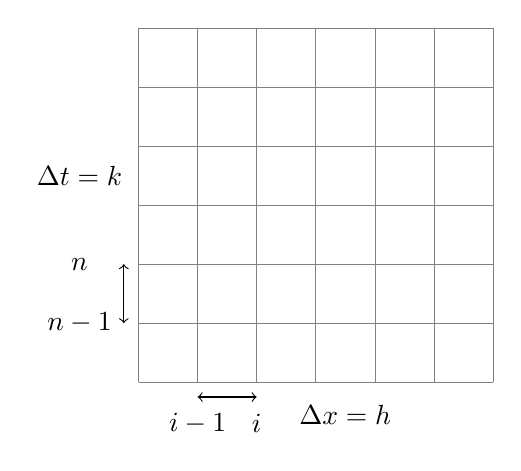
\begin{tikzpicture}[scale=0.75]
      \draw[help lines] (1,1) grid (7,7);

      \draw[<->] (0.75, 2) -- (0.75, 3);
      \node at (0, 4.5) {$\Delta t = k$};
      \node at (0, 2) {$n-1$};
      \node at (0, 3) {$n$};

      \draw[<->] (2, 0.75) -- (3, 0.75);
      \node at (4.5, 0.45) {$\Delta x = h$};
      \node at (2, 0.3) {$i-1$};
      \node at (3, 0.3) {$i$};
    \end{tikzpicture}
    \caption{Mesh Grid example}\label{fde:fig:mesh}
  \end{figure}

  \subsection{Truncation Error}\label{sec:fdes:truncation}
  Suppose that we have some difference equation $D : \mathcal{C}^m \to \mathcal{C}^n$ which is supposed to be an approximation to $L$. Denote $\phi$ be the exact solution to $D(u) = 0$, so $D(\phi) = 0$, and let $\Phi$ be the exact solution to $L(u) = 0$.
\end{document}
